\section{Particle Identification by $dE/dx$}\label{sec:pid}
The specific ionization energy loss, the $dE/dx$, is a function of the
particle momentum magnitude. This property is used
for particle identification. This analysis focuses on particle
identification in the low $p_T$ region. This section describes
the low $p_T$ $dE/dx$ particle identification method in detail.
Extension of particle identification to high $p_T$ is possible
by the Time of Flight (TOF), $t^{TOF}=t^{stop}-t^{start}$ . Due to the low particle multiplicity and lack of signal in VPDs on the outgoing proton side (rapidity gap) in SD events, the $t^{start}$ is not defined precisely.
\begin{figure}[H]
	\centering
	\parbox{0.484\textwidth}{
		\centering
		\begin{subfigure}[b]{\linewidth}{
				\subcaptionbox{\label{fig:nsigmaa}}{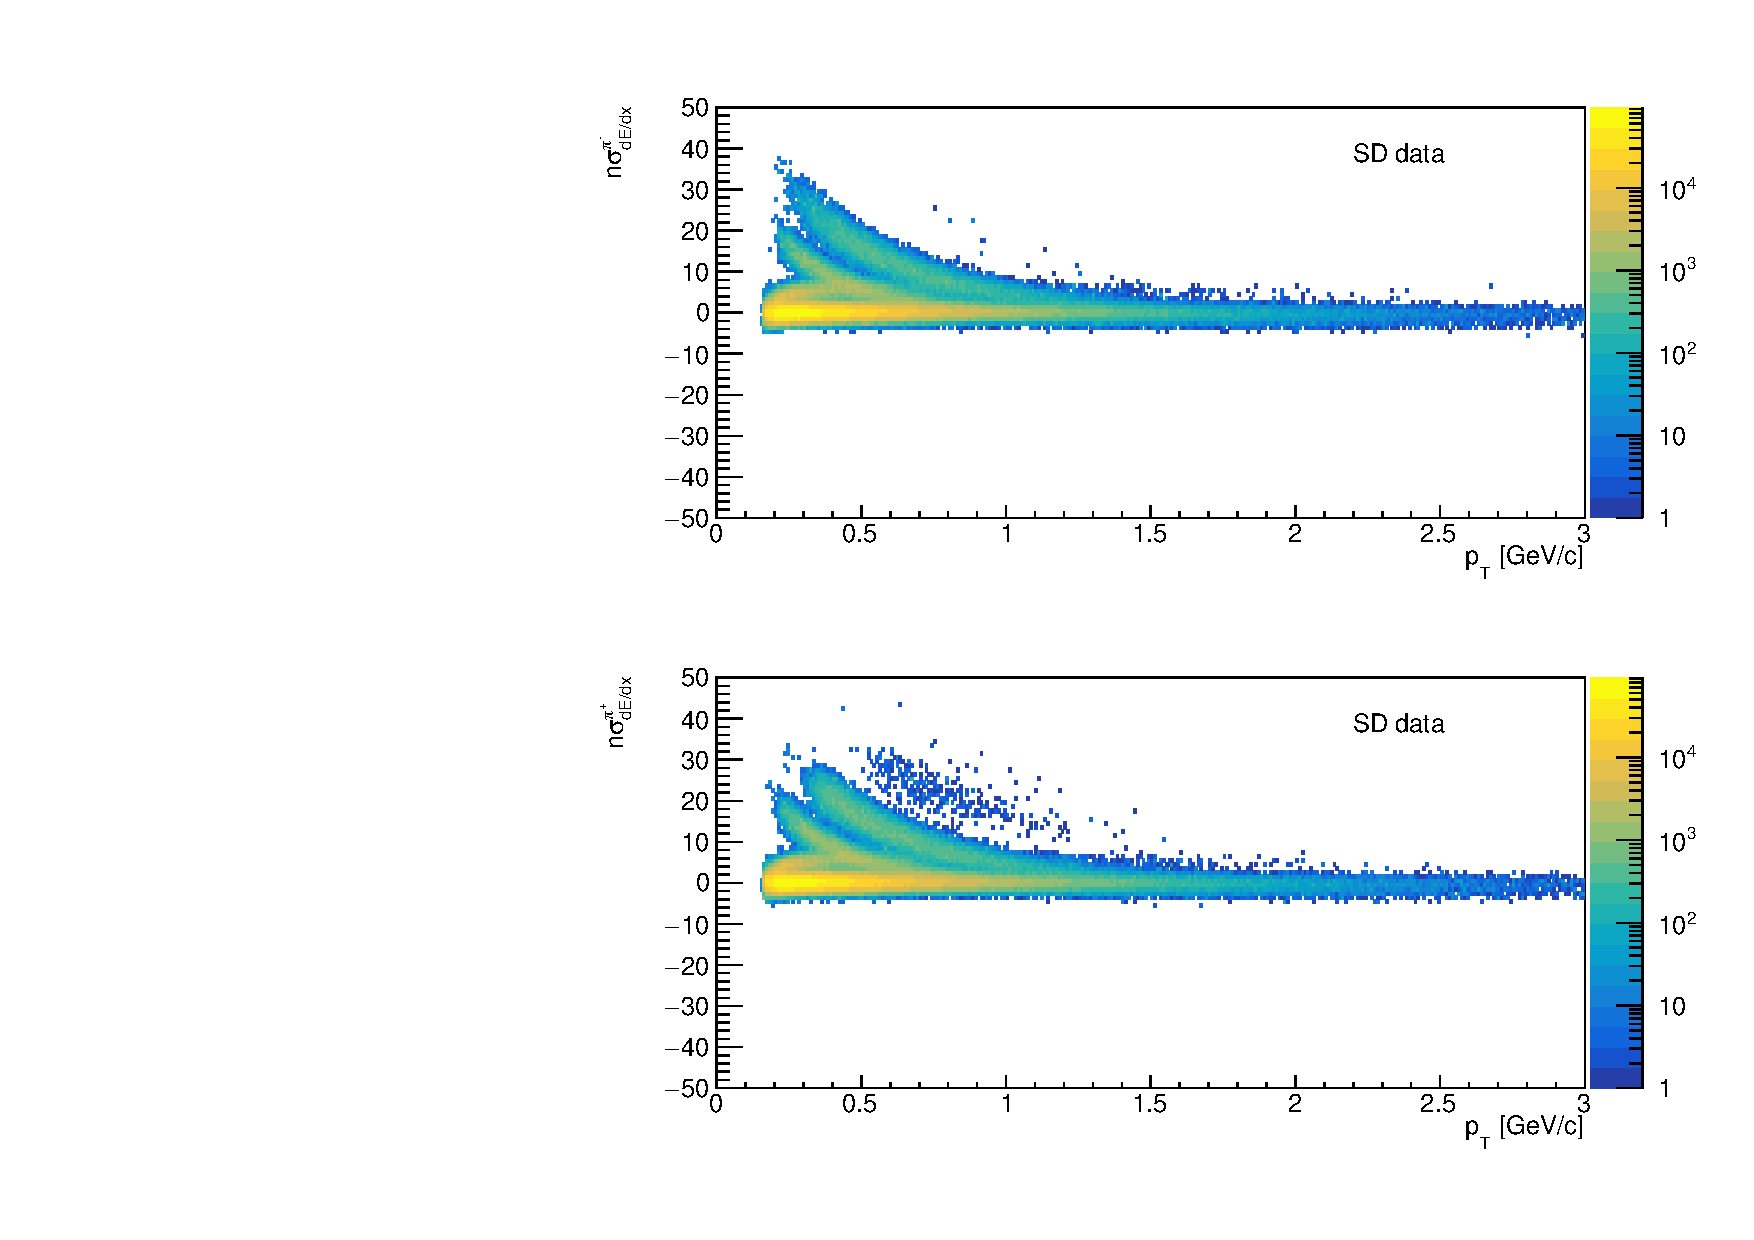
\includegraphics[width=\linewidth, page=1]{graphics/pid/spectraFit_SDT.pdf}}}
		\end{subfigure}
	}
	\quad
	\parbox{0.484\textwidth}{
		\centering
		\begin{subfigure}[b]{\linewidth}{
				\subcaptionbox{\label{fig:nsigmab}}{\includegraphics[width=\linewidth, page=14]{graphics/pid/spectraFit_SDT.pdf}}}
		\end{subfigure}
	}
	\parbox{0.484\textwidth}{
			\centering
			\begin{subfigure}[b]{\linewidth}{
					\subcaptionbox{\label{fig:nsigmac}}{\includegraphics[width=\linewidth, page=21]{graphics/pid/spectraFit_SDT.pdf}}}
			\end{subfigure}
		}
	\caption[The $n\sigma^{i}_{dE/dx}$ variable versus $p_T$ in SD collisions]{The $n\sigma^{i}_{dE/dx}$ variable for particle $i$, where $i=\pi^\pm, K^\pm, p/\bar{p}$, versus $p_T$ in SD collisions. Particles are restricted in $|\eta| < 0.7$
		and corrected for the energy loss (mass of $i$-particle was taken) and vertexing. In
		this narrow pseudo-rapidity slice, $p_T$ is approximately
		equal to $|p|$.}
	\label{fig:nsigma}
\end{figure}

\begin{figure}[H]
	\centering
	\parbox{0.484\textwidth}{
		\centering
		\begin{subfigure}[b]{\linewidth}{
				\subcaptionbox{\label{fig:nsigmafita}}{\includegraphics[width=\linewidth, page=5]{graphics/pid/spectraFit_SDT.pdf}}}
		\end{subfigure}
	}
	\quad
	\parbox{0.484\textwidth}{
		\centering
		\begin{subfigure}[b]{\linewidth}{
				\subcaptionbox{\label{fig:nsigmafitb}}{\includegraphics[width=\linewidth, page=16]{graphics/pid/spectraFit_SDT.pdf}}}
		\end{subfigure}
	}
	\parbox{0.484\textwidth}{
			\centering
			\begin{subfigure}[b]{\linewidth}{
					\subcaptionbox{\label{fig:nsigmafitc}}{\includegraphics[width=\linewidth, page=26]{graphics/pid/spectraFit_SDT.pdf}}}
			\end{subfigure}
		}
	\caption[Distributions of $n\sigma^{\pi^\pm}_{dE/dx}$ for $\pi^\pm$, $n\sigma^{K^\pm}_{dE/dx}$ for $K^\pm$ and $n\sigma^{\bar{p}/p}_{dE/dx}$ for $\bar{p}/p$ in SD collisions]{Distributions of $n\sigma^{\pi^\pm}_{dE/dx}$ for $\pi^\pm$~(a), $n\sigma^{K^\pm}_{dE/dx}$ for $K^\pm$~(b) and $n\sigma^{\bar{p}/p}_{dE/dx}$ for $\bar{p}/p$~(c) in SD collisions. One $p_T$ bin is shown for each particle species. Particles are restricted in $|\eta| < 0.7$ and corrected for the energy loss and vertexing. The curves represent the Gaussian fits to the $n\sigma^{i}_{dE/dx}$ distributions, with individual particle peaks plotted separately.}
	\label{fig:nsigmafit}
\end{figure}